\chapter{Tutorial}

\section{Getting started}

\subsection{Kobold Server}
There are two ways to start and use the Kobold Server - {\it stand-alone} or from
{Eclipse}. In both cases make sure, that you edit the server.properties
file from {\it kobold.server/server.properties} to suite your local
requirements. Under UNIX this file might look similiar to the following
bits:

\begin{verbatim}
# Note storePath is the prefix path for all kobold stores!
kobold.server.storePath=/tmp/
kobold.server.globalMessageStore=global.xml
kobold.server.messageStore=messages.xml
kobold.server.productStore=product.xml
kobold.server.userStore=user.xml
#
java.protocol.handler.pkgs=com.sun.net.ssl.internal.www.protocol
javax.net.debug=all
javax.net.ssl.keyStore=../kobold.common/scripts/keystore
javax.net.ssl.keyStorePassword=kobold1
javax.net.ssl.trustStore=../kobold.common/scripts/truststore
javax.net.ssl.trustStorePassword=kobold1
\end{verbatim}

Under Windows-based systems you've to change the paths into a
DOS-alike format.

In the following table all properties are described in detail:

\begin{tabular}{|l|l|l|}\hline
\textbf{Property} &  \textbf{Description}\\ \hline
kobold.server.storePath  & destination path for files stored by the server \\ \hline
kobold.server.globalMessageStore & file name to store global messages \\
    \hline
kobold.server.messageStore & file name to store pending messages \\
    \hline
kobold.server.productStore & file name to store products and
productlines \\ \hline
kobold.server.userStore & file name to store user data \\ \hline
java.protocol.handler.pkgs & default protocol to commincate \\ \hline
javax.net.debug & debug level of net communication \\ \hline
javax.net.ssl.keyStore & path to your SSL keystore \\ \hline
javax.net.ssl.keyStorePassword & password to access your SSL keystore \\
    \hline
javax.net.ssl.trustStore & path to your SSL truststore \\ \hline
javax.net.ssl.trustStorePassword & password to access your SSL
truststore \\ \hline
\end{tabular}

To start the Kobold server within Eclipse just select 'Run...' in the
'Run' menu from
Eclipse and select the class
{\it kobold.server.SecureKoboldWebServer} with a numerical argument for
the port it should listen for connections. The working directory must be
the directory where your {\it server.properties} are located.

To start the Kobold server from the console just enter following
command within the directory where your {\it server.properties} file is
located:

\begin{verbatim}
java kobold.server.SecureKoboldWebServer 23232
\end{verbatim}

Make sure that your {\it \$CLASSPATH} environment contains all JARs
provided by {\it kobold.common/contrib} beside a Java2 JRE and the Sun
JSSE classes (included by Sun JDK 1.4).

\subsection{Kobold Client Feature Set}
Similiar to the Kobold server, the kobold client feature set contains
a file {\it client.properties} located in {\it
kobold.client.plam/client.properties} which has to be edited to
suite your local requirements.

\begin{verbatim}
# Used for SSL based communication
java.protocol.handler.pkgs=com.sun.net.ssl.internal.www.protocol
javax.net.debug=all
javax.net.ssl.keyStore=/home/garbeam/eclipse/kobold.common/scripts/keystore
javax.net.ssl.keyStorePassword=kobold1
javax.net.ssl.trustStore=/home/garbeam/eclipse/kobold.common/scripts/truststore
javax.net.ssl.trustStorePassword=kobold1
\end{verbatim}

As you can see, it contains the same properties as the {\it
server.properties} file for SSL communication, but since the Kobold
client is independent from the server it has it's own properties.

To start the Kobold client feature set from within Eclipse (which is
currently the only way) just select 'Run...' in the 'Run' menu and
double-click 'Run-time Workbench'. A new configuration is created which you 
can name as you wish (see \ref{run}). 

\begin{figure}[h!]
\begin{center}
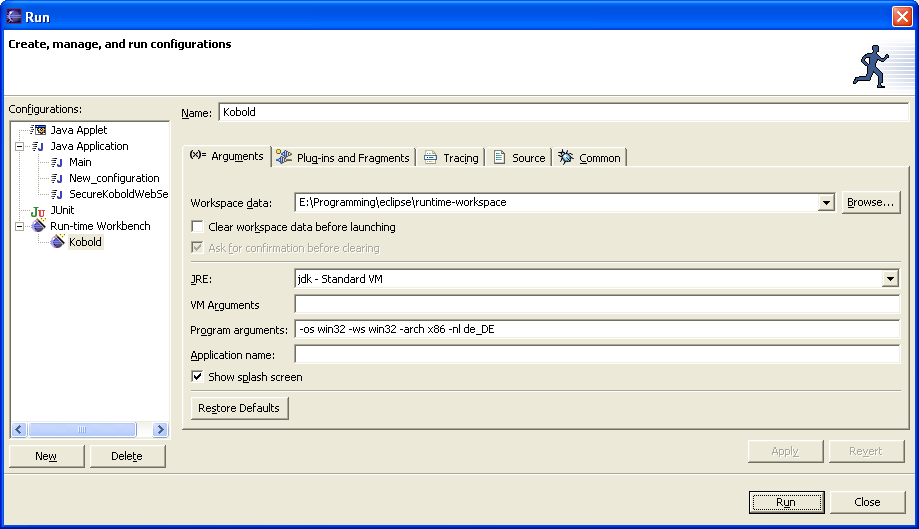
\includegraphics[width=15cm]{run.png}
   \caption{This is how your buildpath should look like}
\label{run}
\end{center}
\end{figure}\par

You've to enter only one VM argument which is needed to locate the {\it
client.properties} file and to suite your local requirements: \par

\begin{verbatim}
-Dkobold.client.configFile=/home/garbeam/eclipse/kobold.client.plam/client.properties
\end{verbatim}

Confirm with 'Run'.

A new Eclipse instance will open with the Kobold feature set enabled.

\section{Checking out a product}

In the File menu select 'New' and then 'Kobold PLAM Project'. The Kobold wizard opens.
Enter enter the url of your Kobold server, your username and password. The press
"test connection". If the test succeeds, the "next" button is enabled and you press it
(see \ref{wizard1}).

\begin{figure}[h!]
\begin{center}
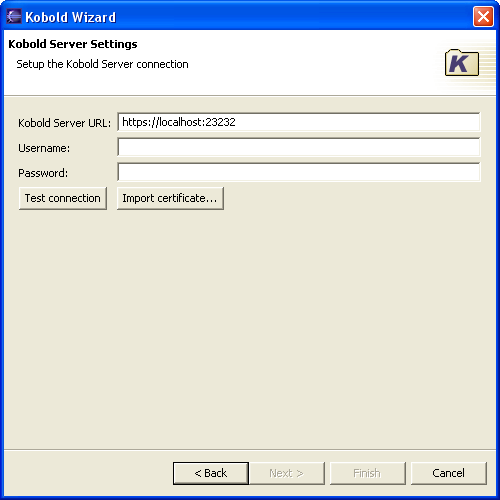
\includegraphics[width=10cm]{wizard1.png}
   \caption{Kobold wizard}
\label{wizard1}
\end{center}
\end{figure}\par

After that you choose the product you want to check out (see \ref{wizard2}).

\begin{figure}[h!]
\begin{center}

\includegraphics[width=10cm]{wizard2.png}
   \caption{Kobold wizard}
\label{wizard2}
\end{center}
\end{figure}\par

In the last step you have to enter the name of the project you want to create (see \ref{wizard3}).

\begin{figure}[h!]
\begin{center}
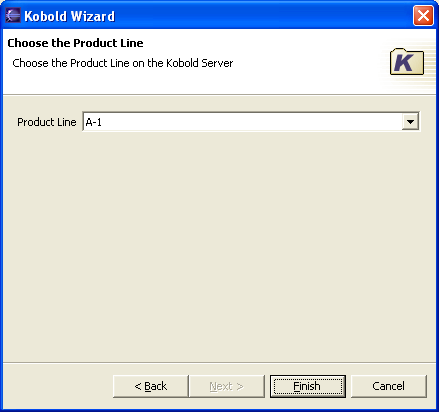
\includegraphics[width=10cm]{wizard3.png}
   \caption{Kobold wizard}
\label{wizard3}
\end{center}
\end{figure}\par

A new project has been created. You can open the different views through the Window menu
and 'show view'. 


\section{Writing a mail}

In the menu of the Workflow View select "new mail". A Workflow window opens where
you can enter your message, the subject and the recipient of the message. Send the
message by pressing the "Send" button. Pressing the "Cancel" button will close the window
without sending your message.

\begin{figure}[h!]
\begin{center}
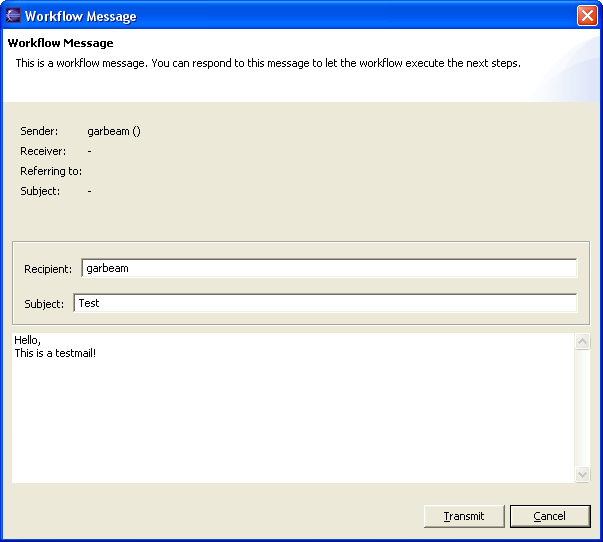
\includegraphics[width=10cm]{writemail.png}
   \caption{Write a new mail}
\label{wizard3}
\end{center}
\end{figure}\par

\section{Answering a mail}

In the Workflow View double-click on the mail you want to answer. A Workflow
window opens where you can see the message text of the mail. Below you can enter
the subject and the text of your reply. Send the answer by pressing the "Send" 
button. Pressing the "Cancel" button will close the window without sending 
your message.

%TODO: Screenshot einf�gen

%\section{Deleting a message}

%Right-click on the message and choose "Delete message" in the context menu.
%Alternatively you can select the message and press "Del" on your keyboard.

\section {Fetching messages}

Select a project. Right-click in the Workflow View or open the corresponding menu. Choose "Fetch message".
Your new messages are being fetched and displayed in the Workflow View.

\section {Filtering the Workflow View}

(still undefined)

\section{Suggesting a file for a Core Group}

In the menu of the Workflow View select "Suggest file for core group". A Workflow
window opens where you can enter the name of the file, its path and the username of the
PE you want to send the message to. You can also enter an additional comment you want 
the PE and PLE to read. Send the message by pressing the "Send" 
button. Pressing the "Cancel" button will close the window without sending 
your message.

\begin{figure}[h!]
\begin{center}
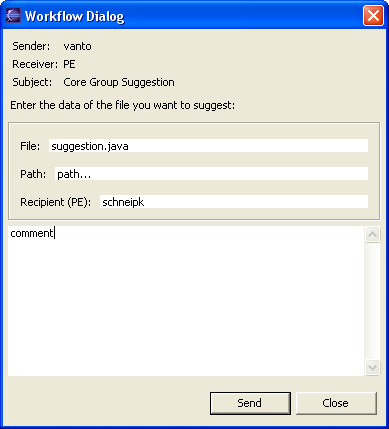
\includegraphics[width=10cm]{core1.png}
   \caption{Suggesting a file for a Core Group}
\label{wizard3}
\end{center}
\end{figure}\par

\section{Dealing with a Core Group suggestion}

In the Workflow View double-click on the Core Group suggestion message. A Workflow
window opens where you can see the message of the programmer (and PE). Below you
can select whether you agree to the suggestion or whether you decline it. You cam a�sp
enter an additional comment if you like. Send the message by pressing the "Send" 
button. Pressing the "Cancel" button will close the window without sending 
your message.\par
Note: The file will not be automatically uploaded and committed. The PLE has to do
this manually.

%TODO: Screenshot einf�gen

\section{Exporting through GXL}

Select the productline, product, component or variant you want to export. In the
menu of the main window select "GXL-Export". A wizard opens where you can choose
whether to create a jar-file of the selected source or not. You should then enter
the path and names of the gxl-file and the jar-file. Alternatively you can enter 
the data through the "save as" dialog. To start the export, press the finish button.
You are able to see the status of your export in the wizard which will close after
the export is finished. If you decide not to do the export, simply press the 
"cancel" button.

%TODO: Screenshot einf�gen

\section{Creating a Core Asset}

In the pallete select the "core asset" tool. Click into the Architecture Editor and
a core asset is inserted. A dialog opens where you can enter the meta data of
the core asset. Per drag+drop you can simply change the size of the core
asset. \par
Note: Core assets can only be inserted on the top-level plane of the Architecture Editor.

%TODO: Screenshot einf�gen

\section{Creating a variant}

In the pallete select the "variant" tool. Click into a core asset or component in 
the Architecture Editor. A variant is inserted. A dialog opens where you can enter the meta data of
the variant. Per drag+drop you can simply change the size of the variant. \par
Note: Variants can only be inserted into core assets or components.

%TODO: Screenshot einf�gen

\section{Creating a component}

In the pallete select the "component" tool. Click into a variant in 
the Architecture Editor. A component is inserted. A dialog opens where you can enter the meta data of
the component. Per drag+drop you can simply change the size of the component. \par
Note: Components can only be inserted into variants.

%TODO: Screenshot einf�gen

\section{Creating a version}

In the pallete select the "version" tool. Click into a variant in 
the Architecture Editor. A version is inserted. A dialog opens where you can enter the meta data of
the version. For each file of the variant you can select the revision number you want to add to the version. 
Per drag+drop you can simply change the size of the version. \par
Note: Versions can only be inserted into variants.

%TODO: Screenshot einf�gen

\section{Creating a meta node}

In the pallete select the "metanode" tool. Click into the Architecture Editor. 
A meta node is inserted. A dialog opens where you can select the type of the node.
Possible types are AND, OR, XOR. 

%TODO: Screenshot einf�gen

\section{Deleting a core asset, component, variant or version}

Right-click on the item you want to delete and choose "delete" in the context
menu. Alternatively you
can select the item and press "Del" on your keyboard. Is the item used in other projects
you will be notified and be able to cancel the deletion process.

%TODO: Screenshot einf�gen

\section{Deleting a meta node}

Right-click on the meta node you want to delete and choose "delete" in the context
menu. Alternatively you
can select the node and press "Del" on your keyboard.

\section{Creating a dependency edge}

In the pallete select the "dependency" tool. Select an item in the Architecture Editor
as the starting point. The next item you select will be the aiming point.

%TODO: Screenshot einf�gen

\section{Creating an exclusion edge}

In the pallete select the "exclude" tool. Select an item in the Architecture Editor
as the starting point. The next item you select will be the aiming point.

%TODO: Screenshot einf�gen

\section{Deleting an edge}

Right-click on the edge you want to delete and choose "delete" in the context menu.
Alternatively you can select the edge and press "Del" on your keyboard.

\section{Marking a component as "deprecated"}
Right-click on the component and choose "mark as deprecated". Alternatively you 
can select the component and press "D" on your keyboard. Deprecated components are
indicated by a small flagg.

%TODO: Screenshot einf�gen

\section{Moving an item}
You can move any item per drag+drop.

\section{Changing the size of an item}
You can change the size of an item per drag+drop.

\section{Filtering the Architecture View}

The toolbar of the Architecture Editor provides you with the following filterings:
\begin{itemize}
	\item Show/hide dependency edges
	\item Show/hide exclusion edges
	\item Show/hide synthetical edges
	\item Show/hide deprecated components
\end{itemize}

%TODO: Screenshot einf�gen

\section{Creating a custom component}

In the pallete select the "custom component" tool. Click into the Architecture 
Editor. A component is inserted. A dialog opens where you can enter the meta data of
the component. Per drag+drop you can simply change the size of the component. \par

%TODO: Screenshot einf�gen

\section{Deleting a custom component}

Right-click on the component you want to delete and choose "delete" in the context
menu. Alternatively you
can select the component and press "Del" on your keyboard. 

\section{Creating a product}
Right-click anywhere and choose "new product" in the context menu. A wizard opens where
you can choose the productline the new product should belong to.

%TODO: Screenshot einf�gen

Press "proceed" 
and choose the CoreAssets for your product. 

%TODO: Screenshot einf�gen

After you press "proceed", you are able
to choose modules of other products from this product line. Press "Finish" and the
new product is created.

\section{Renaming a product}

Right-click on the product and choose "rename product" in the context menu. You can
now enter a new name which will be used in the repository and the product line tree.

%TODO: Screenshot einf�gen

\section{Changing a product}

Right-click on the product and choose "change product". A wizard opens where you can
change the CoreAssets for your product. 

%TODO: Screenshot einf�gen

After you press "proceed", you are able
to choose modules of other products from this product line. Press "Finish" and the changes
are saved.

\section{Setting a product on deprecated}

Right-click on the product and choose "set on deprecated". Confirm your choice in
the upcoming dialog and the product is deprecated. Its modules can no longer be
used in a product.

%TODO: Screenshot einf�gen

\section{Setting a module on deprecated}

Right-click on the product and choose "set on deprecated". Confirm your choice in
the upcoming dialog and the module is deprecated. It can no longer be
used in a product.

%TODO: Screenshot einf�gen

\section{Creating a user}

Right-click on the product the new user shall belong to. In the context menu choose
"new" and then "user". A wizard opens where you can enter the username and the
initial password of the user. 

%TODO: Screenshot einf�gen

After you press "next", you are able to specify the role of the user in the current
project.

%TODO: Screenshot einf�gen

Pressing "next" again finishes the process. The new user is created.

\section{Changing a user role}

Right-click on the corresponding product and choose "change role". A wizard opens.
On the left side you can see a list of all existing users. On 
the right side you can see lists of the product engineers and programmers that
belong to the product. You can switch users from left to right and back by selecting
the user and using
the "<<" and ">>" buttons between the lists. In order to find a specific user in
the left-hand list, enter the initial letters of the user. The list will then show
only those usernames that start with the same letters. Press "Ok" when you are done
and your changes are saved.

%TODO: Screenshot einf�gen

\section{Deleting a user}

(still undefined)

\section{Changing ones password}

(still undefined)